\section{Gegnererkennung}
\begin{frame}
\frametitle{Gegnererkennung}
\framesubtitle{Komponenten}

\begin{figure}
	\begin{tikzpicture}[scale=1, transform shape]
	\def\height{4cm}
	\node[anchor=south west,inner sep=0] (image) at (0,0) {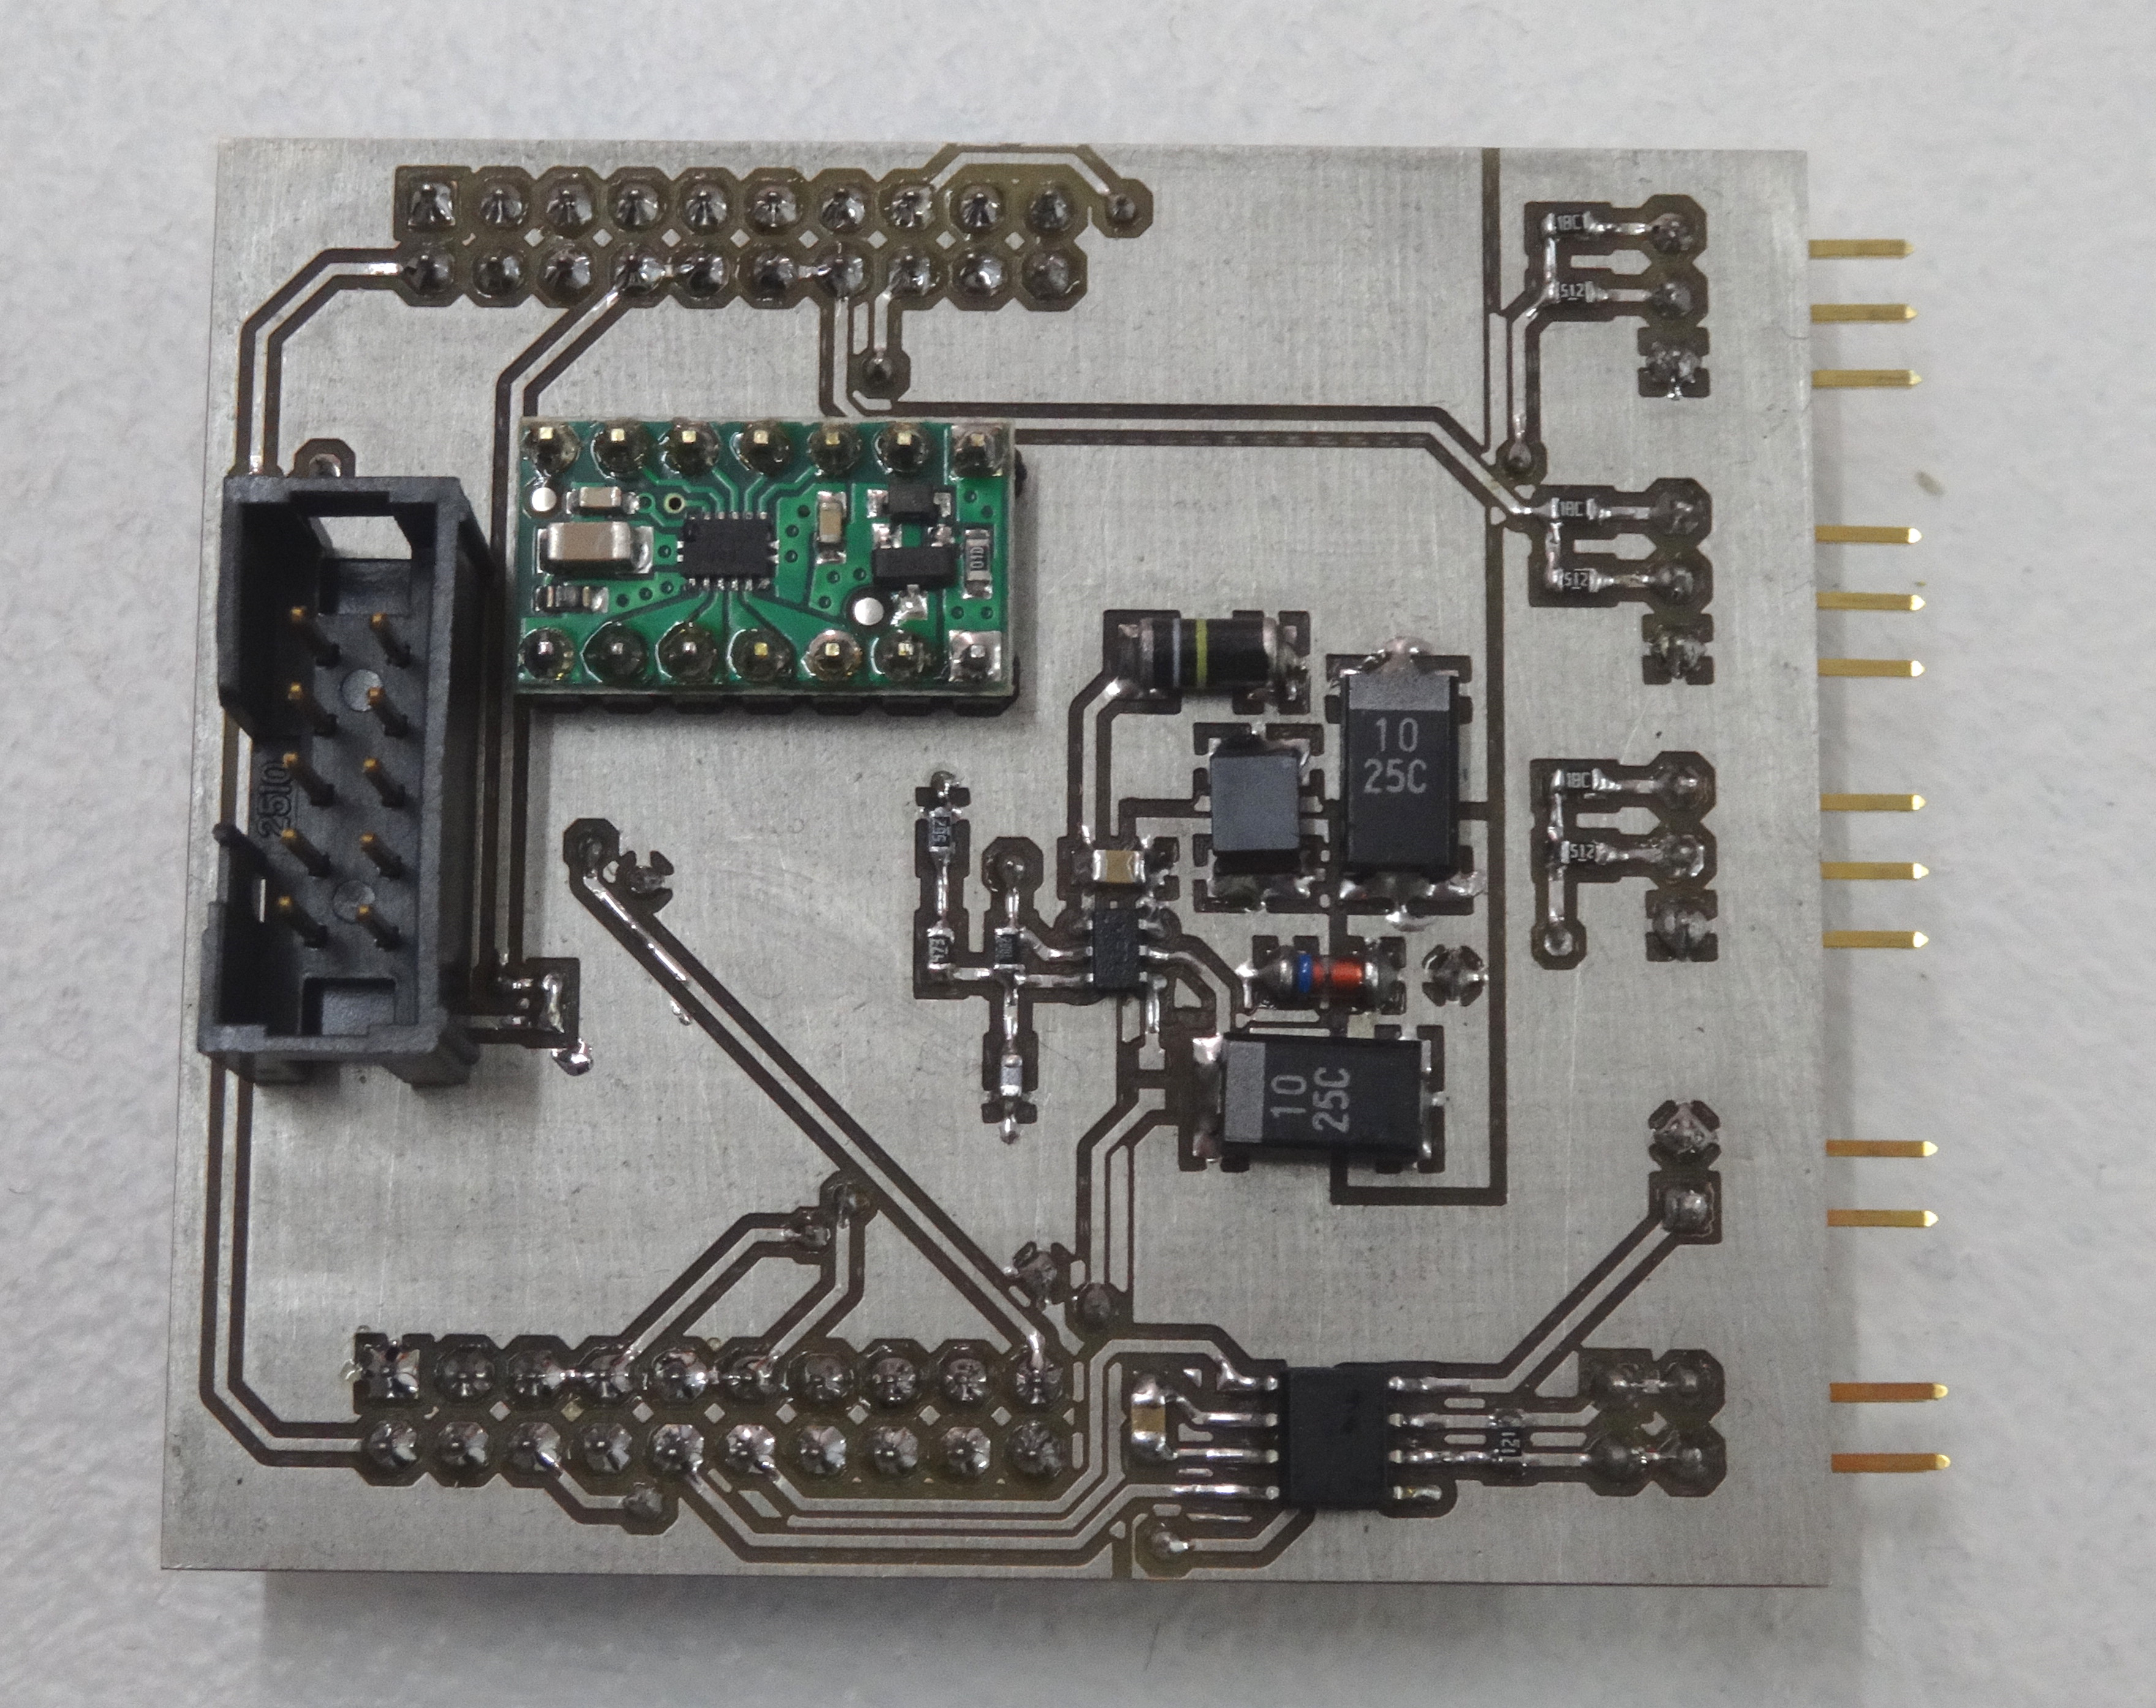
\includegraphics[height=\height] {../images/OD/Adapterboard4.JPG}};
	\begin{scope}[x={(image.south east)},y={(image.north west)}]
		\draw [line width=0.4mm, ->, cGreen] (0.35,1.1) node[left, color=black]{Treiberstufe} -- (0.35,0.75);  
		
		\draw [line width=0.4mm, ->, cGreen] (0.52,1.1) node[right, color=black]{Spannungsregler} -- (0.52, 0.5);
		\draw [line width=0.4mm, ->, cGreen] (0.62,-0.1) node[right, color=black]{CAN-Treiber} -- (0.62, 0.10);
		
		\draw [line width = 0.6mm, -, cRed] (0.15,0.5) to[out = 270, in = 180] (0.5, -0.2);
		\draw [line width = 0.6mm, -, cRed] (0.5, -0.2) -- (1.0, -0.2); 
		%\draw [line width = 0.6mm, -, cRed] (1.0, -0.2) to[out = 0, in = 270] (1.37, 0.1);
		
	\end{scope}
	
	\begin{scope}[xshift=6cm]
		\node[anchor=south west,inner sep=0] (rimage) at (0,0) {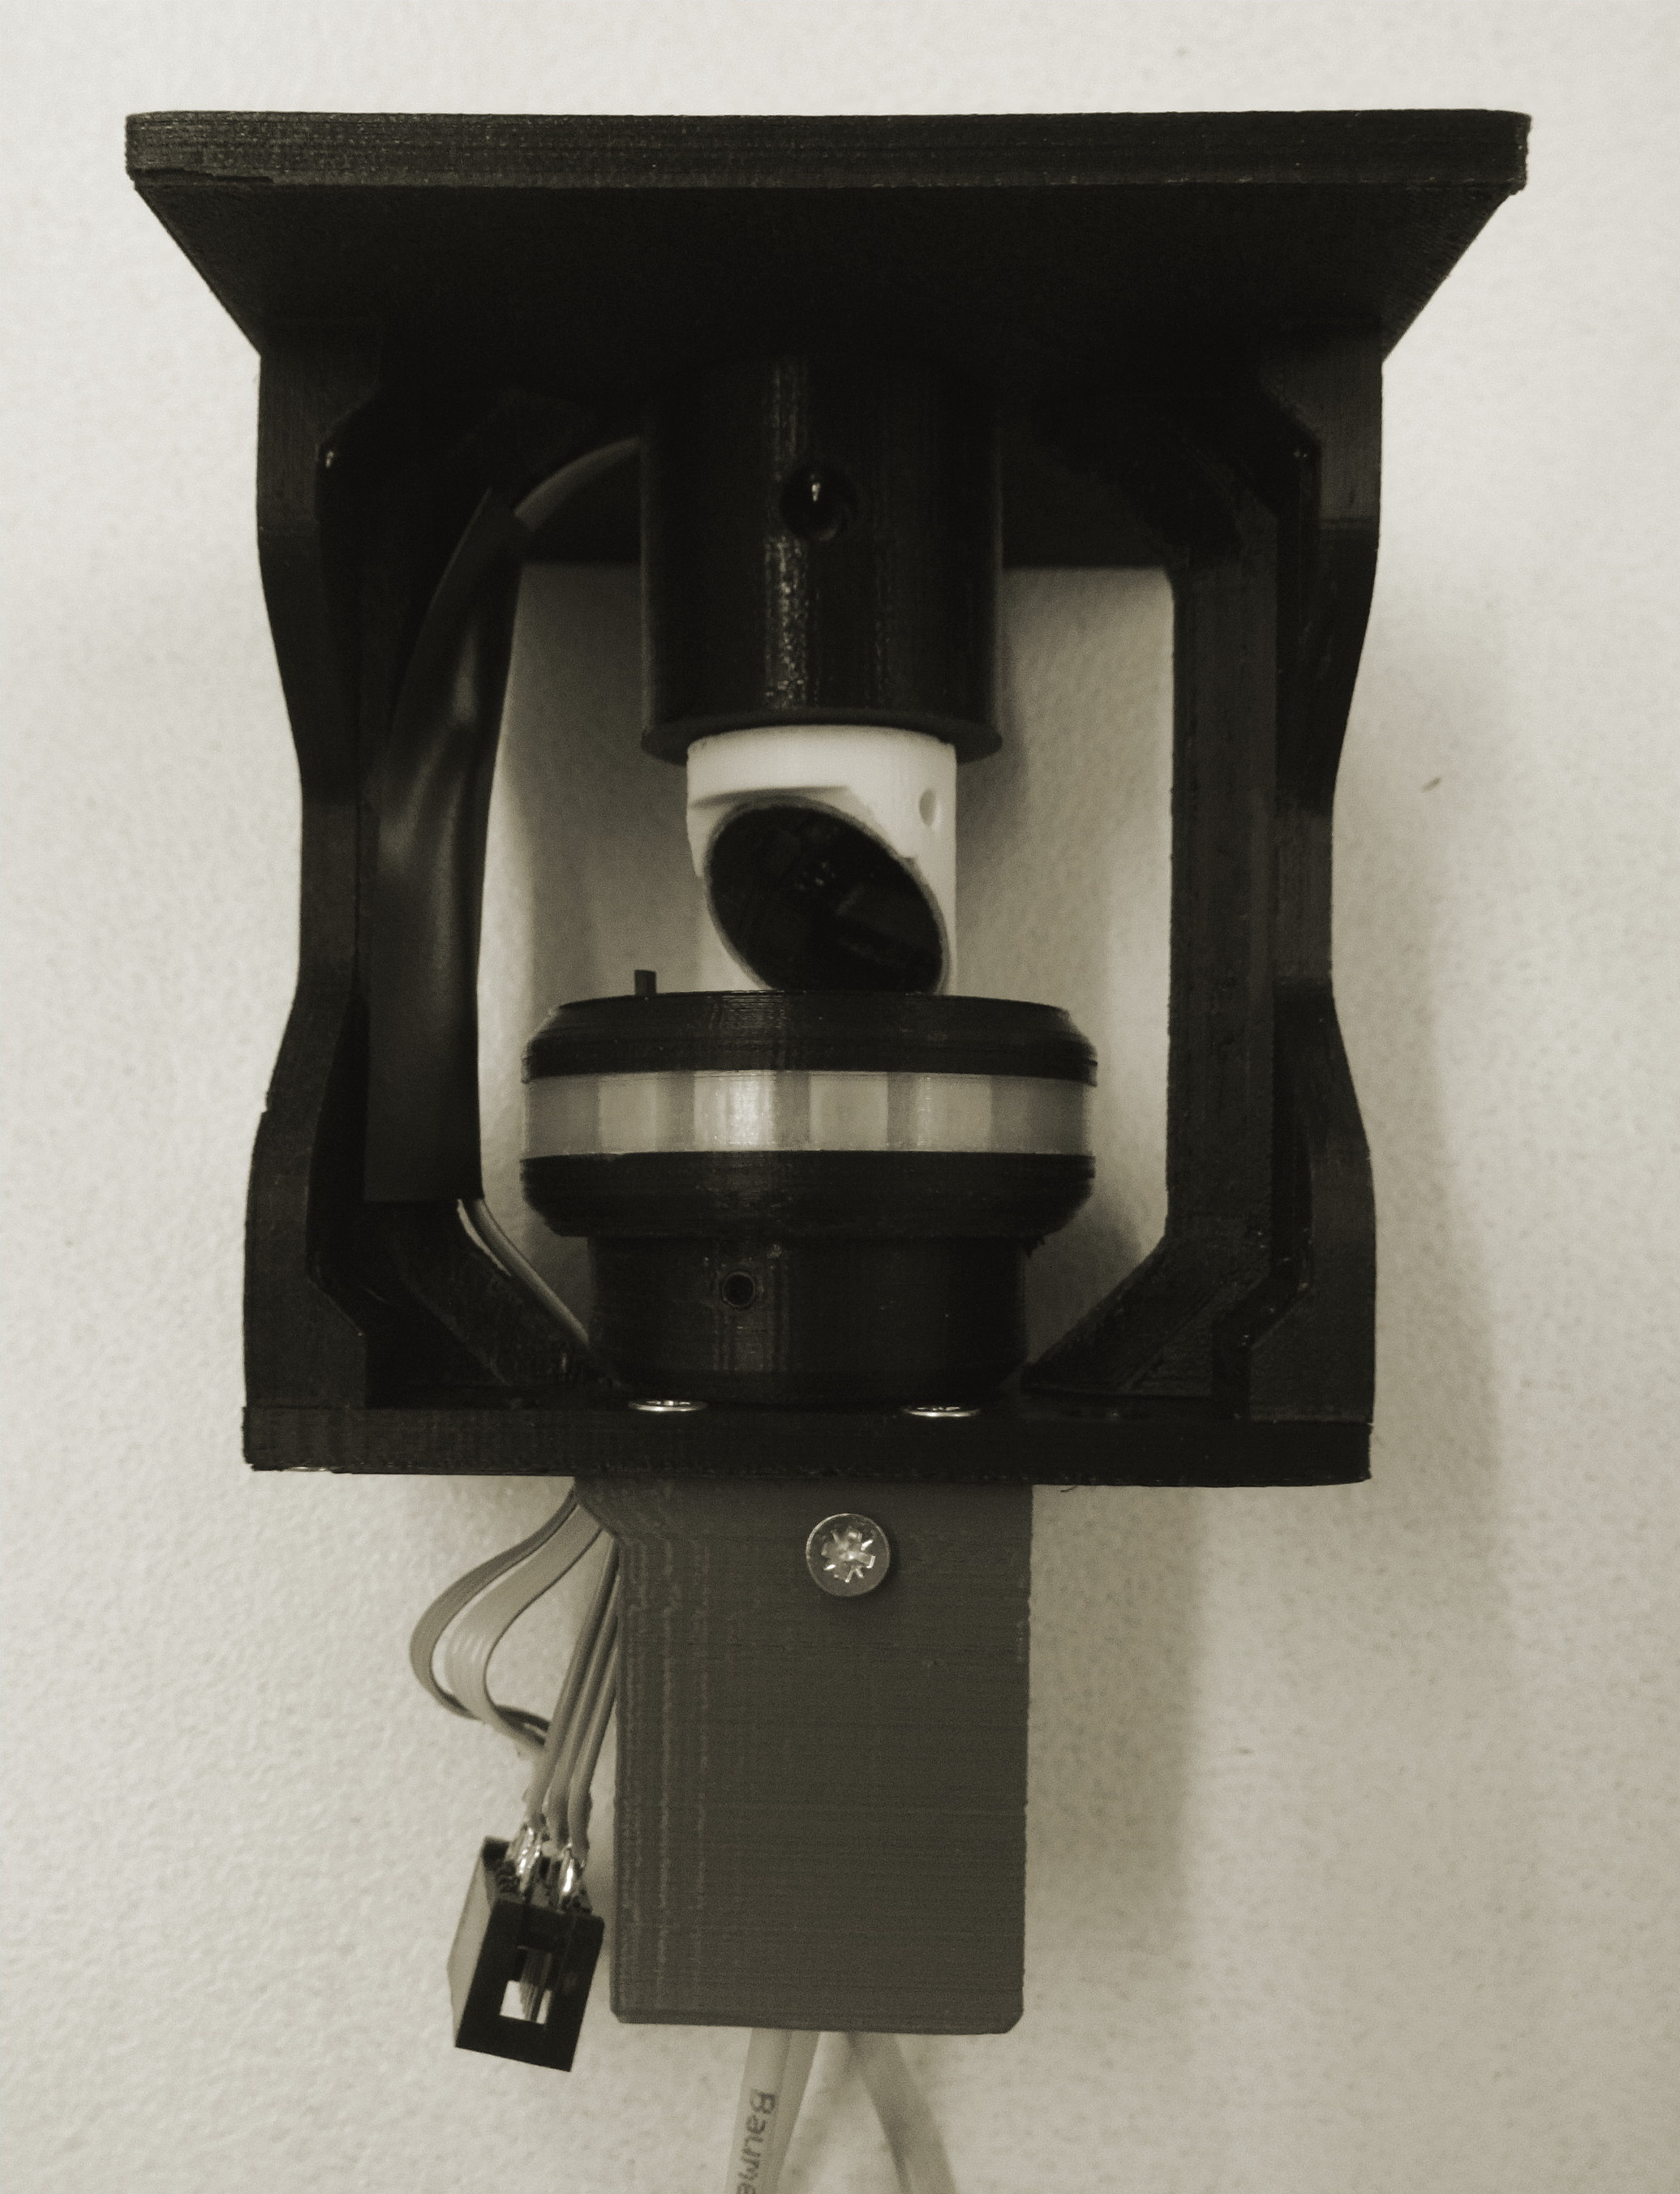
\includegraphics[height=\height] {../images/OD/Kopf3Pres.JPG}};
		\begin{scope}[x={(rimage.south east)},y={(rimage.north west)} ]
		
			\draw [line width=0.4mm, ->, cGreen] (0.5,1.02) node[above, color=black]{Motor und Spiegel} -- (0.5, 0.8);
			\draw [line width=0.4mm, ->, cGreen] (0.55,-0.1) node[right, color=black]{LED-Ring} -- (0.55, 0.4);
			
			\draw [line width = 0.6mm, -, cRed] (-0.32, -0.1985) to[out = 0, in = 270] (0.32, 0.1);
			\draw [line width = 0.4mm, -, cRed] (-0.49, 0.87) -- (-0.49, 0.44);
			\draw [line width = 0.6mm, -, cRed] (-0.49, 0.655) to[out = 0, in = 90] (-0.2, 0.44);
			\draw [line width = 0.6mm, -, cRed] (-0.2, 0.44) -- (-0.2, 0.0);
			\draw [line width = 0.6mm, -, cRed] (-0.2, 0.0) to[out = 270, in = 270] (0.5, 0.0);
		
		\end{scope}
	\end{scope}
	\end{tikzpicture}	
\end{figure}

\end{frame}

\begin{frame}
	\frametitle{Gegnererkennung}
	\framesubtitle{Ausmessung Spiegelhalter}
	
	\begin{figure}
		\centering
		\begin{tikzpicture}[y=-1cm, scale=0.5, transform shape]
		%near right
		\draw [draw=cRed, fill=clRed, fill opacity=0.3] (300:0.6) -- (300:1.95) -- (330:1.65) -- (0:1.6) -- (30:1.8) -- (60:2.4) -- (60:0.8) -- (30:0.65) -- (0:0.5) -- (330:0.5) -- (300:0.6);		
		%middle right
		\draw [draw=cBlue, fill=clBlue, fill opacity=0.3] (300:0.95) -- (330:0.93) -- (0:0.88) -- (30:0.85) -- (60:0.8) -- (60:2.75) -- (30:3.1) -- (0:3.05) -- (330:3.1) -- (300:3.05) -- (300:0.95);
		%middle left
		\draw [draw=cBlue, fill=clBlue, fill opacity=0.3] (120:0.73) -- (150:0.73) -- (180:0.75) -- (210:0.78) -- (240:0.88) -- (240:2.65) -- (210:2.8) -- (180:2.65) -- (150:2.35) -- (120:2.35) -- (120:0.73);
		%far right
		\draw [draw=cGreen, fill=clGreen, fill opacity=0.3] (300:1.25) -- (330:1.25) -- (0:1.1) -- (30:1) -- (60:0.88) -- (60:3.15) -- (30:4.2) -- (0:4.95) -- (330:4.9) -- (300:5) -- (300:1.5);
		
		%far left
		\draw [draw=cGreen, fill=clGreen, fill opacity=0.3] (120:0.65) -- (150:0.55) -- (180:0.6) -- (210:0.7) -- (240:0.83) -- (240:2.9) -- (210:2.25) -- (180:2) -- (150:1.75) -- (120:1.85) -- (120:0.65);
		%middle left
		\draw [draw=cBlue, fill=clBlue, fill opacity=0.3] (120:0.73) -- (150:0.73) -- (180:0.75) -- (210:0.78) -- (240:0.88) -- (240:2.65) -- (210:2.8) -- (180:2.65) -- (150:2.35) -- (120:2.35) -- (120:0.73);
		% near left
		\draw [draw=cRed, fill=clRed, fill opacity=0.3] (120:1.4) -- (150:1.7) -- (180:1.75) -- (210:1.65) -- (240:1.25) -- (240:4.25) -- (210:5) -- (180:5) -- (150:5) -- (120:5) -- (120:1.4);
		
		%draw Coordinate System
		\foreach \phi/\t in {0/90,30/120,60/150,90/180,120/210,150/240,180/270,210/300,240/330,270/0,300/30,330/60}
		{
			\draw [color=cGray] (0,0) -- (\phi:5.5);
			\node [fill=white] at (\phi:5.7) {\t°};
		}
		\foreach \r in {1,1.5,2,2.5,3,3.5,4,4.5,5}
		{
			\draw [color=cGray] (0,0) circle (\r);
		}
		\foreach \t/\x in {200/1,400/2,600/3,800/4,1000/5}
		{
			\node [fill=white, rounded corners=2mm] at (270:\x) {\t};
		}
		
		\draw [thick, ->] (0:7) -- (0:9) node[pos=0.5, above] {Vorwärts};
		
		\end{tikzpicture}
	\end{figure}

\end{frame}